%label:"thm:viterboRestriction"
%author:JeffHicks
%name:"Viterbo restriction"
%type:"theorem"
%source:"viterbo1999functors"


    \label{thm:viterboRestriction}
    Let $X_0\subset X$ be a Liouville subdomain. Then there is a restriction map $\SH(X)\to \SH(X_0)$, which is a unital ring homomorphism. Furthermore, we have a commutative diagram
    %tag:000X
%label:"dig:viterboSuggestive"
%type:"diagram"
%parent:thm:viterboRestriction
%author:JeffHicks

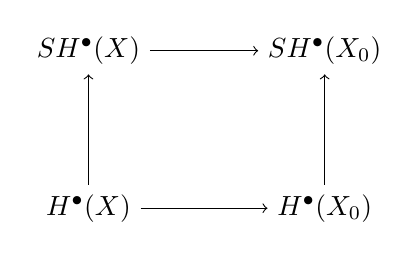
\begin{tikzpicture}

    \node (v3) at (-2,1) {$SH^\bullet(X)$};
    \node (v4) at (1,1) {$SH^\bullet(X_0)$};
    \node (v1) at (-2,-1) {$H^\bullet(X)$};
    \node (v2) at (1,-1) {$H^\bullet(X_0)$};
    \draw  (v1) edge[->] (v2);
    \draw  (v1) edge[->] (v3);
    \draw  (v3) edge[->] (v4);
    \draw  (v2) edge[->] (v4);
\end{tikzpicture}
    where the horizontal maps are given by \cref{prp:homologyIncludesIntoSH}.
